% LaTeX Präsentationsvorlage (2013) der TU Graz, rev12, 2013/01/31
% !TeX encoding = UTF-8
\documentclass{beamer}
% \documentclass[aspectratio=169]{beamer}
% \usetheme{tugraz2013}
% \usetheme[notes]{tugraz2013}
\usepackage{../common/beamerthemetugraz2013}
\usepackage{color}
\usepackage{multicol}
\usepackage{bbding}
\usepackage{wasysym}
\usepackage{caption}
% \usepackage{minted}

\usepackage{listings}
\usepackage{xcolor}

\definecolor{codegreen}{rgb}{0,0.6,0}
\definecolor{codegray}{rgb}{0.5,0.5,0.5}
\definecolor{codepurple}{rgb}{0.58,0,0.82}
\definecolor{backcolour}{rgb}{0.95,0.95,0.92}
\lstdefinestyle{mystyle}{
    backgroundcolor=\color{backcolour},   
    commentstyle=\color{codegreen},
    keywordstyle=\color{magenta},
    numberstyle=\tiny\color{codegray},
    stringstyle=\color{codepurple},
    basicstyle=\ttfamily\footnotesize,
    breakatwhitespace=false,         
    breaklines=true,                 
    captionpos=b,                    
    keepspaces=true,                 
    numbers=left,                    
    numbersep=5pt,                  
    showspaces=false,                
    showstringspaces=false,
    showtabs=false,                  
    tabsize=2
}

\lstset{style=mystyle}

\usepackage{picture}
\usepackage{rotating}
\definecolor{darkred}{rgb}{0.85,0.16,0.0}
\definecolor{darkgreen}{rgb}{0.16,0.70,0.27}

\usepackage{xcolor}


\newcommand{\hrefu}[2]{\underline{\href{#1}{#2}}}
\newcommand{\hyperlinku}[2]{\underline{\hyperlink{#1}{#2}}}
\newcommand{\smallurl}[1]{%
  \begin{flushleft}
    \tiny\url{#1}
  \end{flushleft}
}
\newcommand{\smalltext}[1]{%
  \begin{flushleft}
    \tiny{#1}
  \end{flushleft}
}
\newcommand{\red}[1]{{\color{red} #1}}
\newcommand{\blue}[1]{{\color{blue} #1}}
\newcommand{\darkgreen}[1]{\textcolor{darkgreen}{#1}}
\newcommand{\darkred}[1]{\textcolor{darkred}{#1}}

\newcommand*{\vpointer}{\vcenter{\hbox{\scalebox{1.5}{\large\pointer}}}}

\newcommand{\be}[1]{\begin{equation} \label{#1}}
\newcommand{\ee}{\end{equation}}
\newcommand{\bea}[1]{\begin{eqnarray} \label{#1}}
\newcommand{\eea}{\end{eqnarray}}
\newcommand{\bean}{\begin{eqnarray*}}
\newcommand{\eean}{\end{eqnarray*}}

\newcommand{\non}{\nonumber\\}
\newcommand{\eq}[1]{(\ref{#1})}
\newcommand{\difp}[2]{\frac{\partial #1}{\partial #2}}
\newcommand{\br}{{\bf r}}
\newcommand{\bR}{{\bf R}}
\newcommand{\bA}{{\bf A}}
\newcommand{\bB}{{\bf B}}
\newcommand{\bE}{{\bf E}}
\newcommand{\bm}{{\bf m}}
%\renewcommand{\bm}{{\bf m}}
\newcommand{\bn}{{\bf n}}
\newcommand{\bN}{{\bf N}}
\newcommand{\bp}{{\bf p}}
\newcommand{\bP}{{\bf P}}
\newcommand{\bF}{{\bf F}}
\newcommand{\by}{{\bf y}}
\newcommand{\bz}{{\bf z}}
\newcommand{\bZ}{{\bf Z}}
\newcommand{\bV}{{\bf V}}
\newcommand{\bv}{{\bf v}}
\newcommand{\bu}{{\bf u}}
\newcommand{\bx}{{\bf x}}
\newcommand{\bX}{{\bf X}}
\newcommand{\bW}{{\bf W}}
\newcommand{\bJ}{{\bf J}}
\newcommand{\bj}{{\bf j}}
\newcommand{\bk}{{\bf k}}
\newcommand{\bTheta}{{\bf \Theta}}
\newcommand{\btheta}{{\boldsymbol\theta}}
\newcommand{\bOmega}{{\bf \Omega}}
\newcommand{\bomega}{{\boldsymbol\omega}}
\newcommand{\brho}{{\boldsymbol\rho}}
\newcommand{\rd}{{\rm d}}
\newcommand{\rJ}{{\rm J}}
\newcommand{\ph}{{\varphi}}
\newcommand{\te}{\theta}
\newcommand{\tht}{\vartheta}
\newcommand{\vpar}{v_\parallel}
\newcommand{\vparkb}{v_{\parallel k b}}
\newcommand{\vparkm}{v_{\parallel k m}}
\newcommand{\Jpar}{J_\parallel}
\newcommand{\ppar}{p_\parallel}
\newcommand{\Bpstar}{B_\parallel^*}
\newcommand{\intpi}{\int\limits_{0}^{2\pi}}
\newcommand{\summ}{\sum \limits_{m=-\infty}^\infty}
\newcommand{\tb}{\tau_b(\uv)}
\newcommand{\bh}{{\bf h}}
\newcommand{\cE}{{\cal E}}
\newcommand{\bsigma}{{\boldsymbol\sigma}}
\newcommand{\bS}{{\mathbf S}}
\newcommand{\bI}{{\mathbf I}}
\newcommand{\odtwo}[2]{\frac{\rd #1}{\rd #2}}
\newcommand{\pdone}[1]{\frac{\partial}{\partial #1}}
\newcommand{\pdtwo}[2]{\frac{\partial #1}{\partial #2}}
\newcommand{\ds}{\displaystyle} % commands


%% Titelblatt-Einstellungen
\title[]
{Python 00}
\author[E.~Wachmann]{\scriptsize Elias Wachmann
}
\date{2024} % \today für heutiges Datum verwenden
\institute[Institute of Theoretical and Computational Physics]
{
}
\instituteurl{www.tugraz.at}
% \institutelogo{kurz.pdf}
%~ \additionallogo{merged_logos}
\AtBeginSection[]{
  \begin{frame}
  \vfill
  \centering
  \begin{beamercolorbox}[sep=8pt,center,shadow=true,rounded=true]{title}
    \usebeamerfont{title}\insertsectionhead\par%
  \end{beamercolorbox}
  \vfill
  \end{frame}
}
%%%%%%%%%%%%%%%%%%%%%%%%%%%%%%%%%%%%%%%%%%%%%%%%%%%%%%%%%%%%%%%%%%%%%%%%%%%%
\begin{document}
%%%%%%%%%%%%%%%%%%%%%%%%%%%%%%%%%%%%%%%%%%%%%%%%%%%%%%%%%%%%%%%%%%%%%%%%%%%%
\titleframe


\begin{frame}
  \vspace*{\fill}
  \begin{center}
    \begin{quote}
        ``The magic of computing begins with 0, a simple binary digit that serves as a powerful reminder that even the smallest building blocks can create wonders.''
    \end{quote}
\end{center}
\vspace*{\fill}
\end{frame}

\begin{frame}
\frametitle{Content}
  \tableofcontents
\end{frame}

%%%%%%%%%%%%%%%%%%%%%%%%%%%%%%%%%%%%%%%%%%%%%%%%%%%%%%%%%%%%%%%%%%%%%%%%%%%%
\label{sec:intro}
\section{Introduction}
\begin{frame}
  \frametitle{Introduction}
  This course is designed to teach you the basics of programming in \hrefu{https://www.python.org/}{Python}.\\
  \vspace{0.5cm}
  However, before we start, we need to understand how computers work. This slide deck will give you a brief introduction to the topic. 
\end{frame}
\begin{frame}
  \frametitle{Introduction}
  The slide decks will include lots of examples for various concepts. \\
  Feel free to try them out \textbf{yourself}, since this is the best way to learn programming.\\
  \vspace{0.5cm}
  By the end of this course, you'll have a solid foundation in Python programming and be ready to take on more advanced courses and real-world projects!
\end{frame}
%%%%%%%%%%%%%%%%%%%%%%%%%%%%%%%%%%%%%%%%%%%%%%%%%%%%%%%%%%%%%%%%%%%%%%%%%%%%
\label{sec:binary_numbers}
\section{Binary numbers}
\begin{frame}
  \frametitle{Binary Representation}
  Binary representation is a method of representing numbers using only two digits, typically 0 and 1. It is commonly used in computer systems.\
  
  For example, the decimal number 5 can be represented in binary as \textbf{$101$}, where the rightmost digit represents the \textbf{$2^0$} place, the next digit represents the \textbf{$2^1$} place, and so on.\
\end{frame}
\begin{frame}
  \frametitle{Binary Representation of 42}
  To convert the decimal number 42 to binary, we can use the following method:
  
  \vspace{0.5cm}
  
  \begin{tabular}{c c c c c c c c }
  &42 & 21 & 10 & 5 & 2 & 1 & 0 \\ 
  &÷ 2 & ÷ 2 & ÷ 2 & ÷ 2 & ÷ 2 & ÷ 2 & \\\hline
  &21 & 10 & 5 & 2 & 1 & 0 & \\
  Remainder: & 0 &  1 &  0 &  1 &  0 &  1 & \\
  \end{tabular}
  \vspace{0.5cm}

  Reading the remainders from right to left, we get the binary representation of 42 as \texttt{0b00101010}.\\Or: $2^5 + 2^3 + 2^1 + 2^0 = 32 + 8 + 2= 42$.	
  \end{frame}
  \begin{frame}
    \frametitle{Representing Negative Numbers}
    
    Negative numbers can be represented in binary using a method called \hrefu{https://en.wikipedia.org/wiki/Two\%27s_complement}{\textbf{Two's Complement}}:
    
    \vspace{0.5cm}
    
    \textbf{Step 1:} Write down the binary representation of the positive number.
    
    \textbf{Step 2:} Invert all the bits (change 0s to 1s and 1s to 0s).
    
    \textbf{Step 3:} Add 1 to the result from step 2.
    
    \vspace{0.5cm}
    $42 \xrightarrow{1}$ \texttt{0b00101010} $\xrightarrow{2}$ \texttt{0b11010101} $\xrightarrow{3}$ \texttt{0b11010110} $=-42$
\end{frame}
\begin{frame}
  \frametitle{Some Examples}
  0 to 15 in binary:
\begin{center}
  \begin{tabular}{ | c | c | c | c | }
    \hline
    Decimal & Binary & Decimal & Binary \\ \hline
    0 & \texttt{0b0000} & 8  & \texttt{0b1000} \\ \hline
    1 & \texttt{0b0001} & 9  & \texttt{0b1001} \\ \hline
    2 & \texttt{0b0010} & 10 & \texttt{0b1010} \\ \hline
    3 & \texttt{0b0011} & 11 & \texttt{0b1011} \\ \hline
    4 & \texttt{0b0100} & 12 & \texttt{0b1100} \\ \hline
    5 & \texttt{0b0101} & 13 & \texttt{0b1101} \\ \hline
    6 & \texttt{0b0110} & 14 & \texttt{0b1110} \\ \hline
    7 & \texttt{0b0111} & 15 & \texttt{0b1111} \\ \hline
  \end{tabular}
\end{center}
\end{frame}
\label{sec:hexadecimal_numbers}
\section{Hexadecimal numbers}
\begin{frame}
\frametitle{Hexadecimal Representation}
Hexadecimal representation is a method of representing numbers using 16 distinct symbols, typically 0-9 and A-F. It is commonly used in computer systems as a more compact representation of binary numbers.

For example, the decimal number 42 can be represented in hexadecimal as \textbf{$2A$}, where the rightmost digit represents the \textbf{$16^0$} place and the next digit represents the \textbf{$16^1$} place.
\end{frame}
\begin{frame}
\frametitle{Hexadecimal Representation of 42}
To convert the decimal number 42 to hexadecimal, we can use the following method:

\vspace{0.5cm}

\begin{tabular}{c c c c }
&42 & 2 & 0\\
&÷ 16 & ÷ 16 &\\ \hline
&2 & 0 &\\
Remainder: & 10 & 2 &\\
\end{tabular}
\vspace{0.5cm}

Reading the remainders from right to left, we get the hexadecimal representation of 42 as \texttt{0x2A}.\\Or: $16^1 + 10^0 = 32 + 10 = 42$.
\end{frame}

\begin{frame}
\frametitle{Converting Hexadecimal to Binary}
To convert a hexadecimal number to binary, each digit can be replaced by its 4-bit binary equivalent.

\vspace{0.5cm}

For example, to convert \texttt{0x2A} to binary:

\vspace{0.5cm}

\begin{tabular}{c c c c}
2 & $\rightarrow$ & \texttt{0010} & \\
A & $\rightarrow$ & \texttt{1010} & \\
\end{tabular}

\vspace{0.5cm}

Concatenating the binary equivalents, we get \texttt{0b00101010}.
\end{frame}
\begin{frame}
\frametitle{Some Examples}
0 to 15 in hexadecimal:
\begin{center}
\begin{tabular}{ | c | c | c | c | }
\hline
Decimal & Hexadecimal & Decimal & Hexadecimal \\ \hline
0 & \texttt{0x0} & 8 & \texttt{0x8} \\ \hline
1 & \texttt{0x1} & 9 & \texttt{0x9} \\ \hline
2 & \texttt{0x2} & 10 & \texttt{0xA} \\ \hline
3 & \texttt{0x3} & 11 & \texttt{0xB} \\ \hline
4 & \texttt{0x4} & 12 & \texttt{0xC} \\ \hline
5 & \texttt{0x5} & 13 & \texttt{0xD} \\ \hline
6 & \texttt{0x6} & 14 & \texttt{0xE} \\ \hline
7 & \texttt{0x7} & 15 & \texttt{0xF} \\ \hline
\end{tabular}
\end{center}
\end{frame}


\label{sec:how_do_computers_work}
\section{How do Computers work}
\begin{frame}
  \frametitle{Bits and Bytes}
  Computers store all information as a series of 0s and 1s. These 0s and 1s are called \textbf{bits}. A group of 8 bits is called a \textbf{byte}.\\
  \vspace{0.5cm}
  For example, the decimal number 42 can be represented as the byte \texttt{0b00101010}. 
  \vspace{0.5cm}

  % \begin{center}
  %   \includegraphics[width=0.6\textwidth]{fig/binary\_42.pdf}
  % \end{center}
\end{frame}
\begin{frame}
  \frametitle{Bit storage}
  How do computers store bits?\\
  \begin{center}
    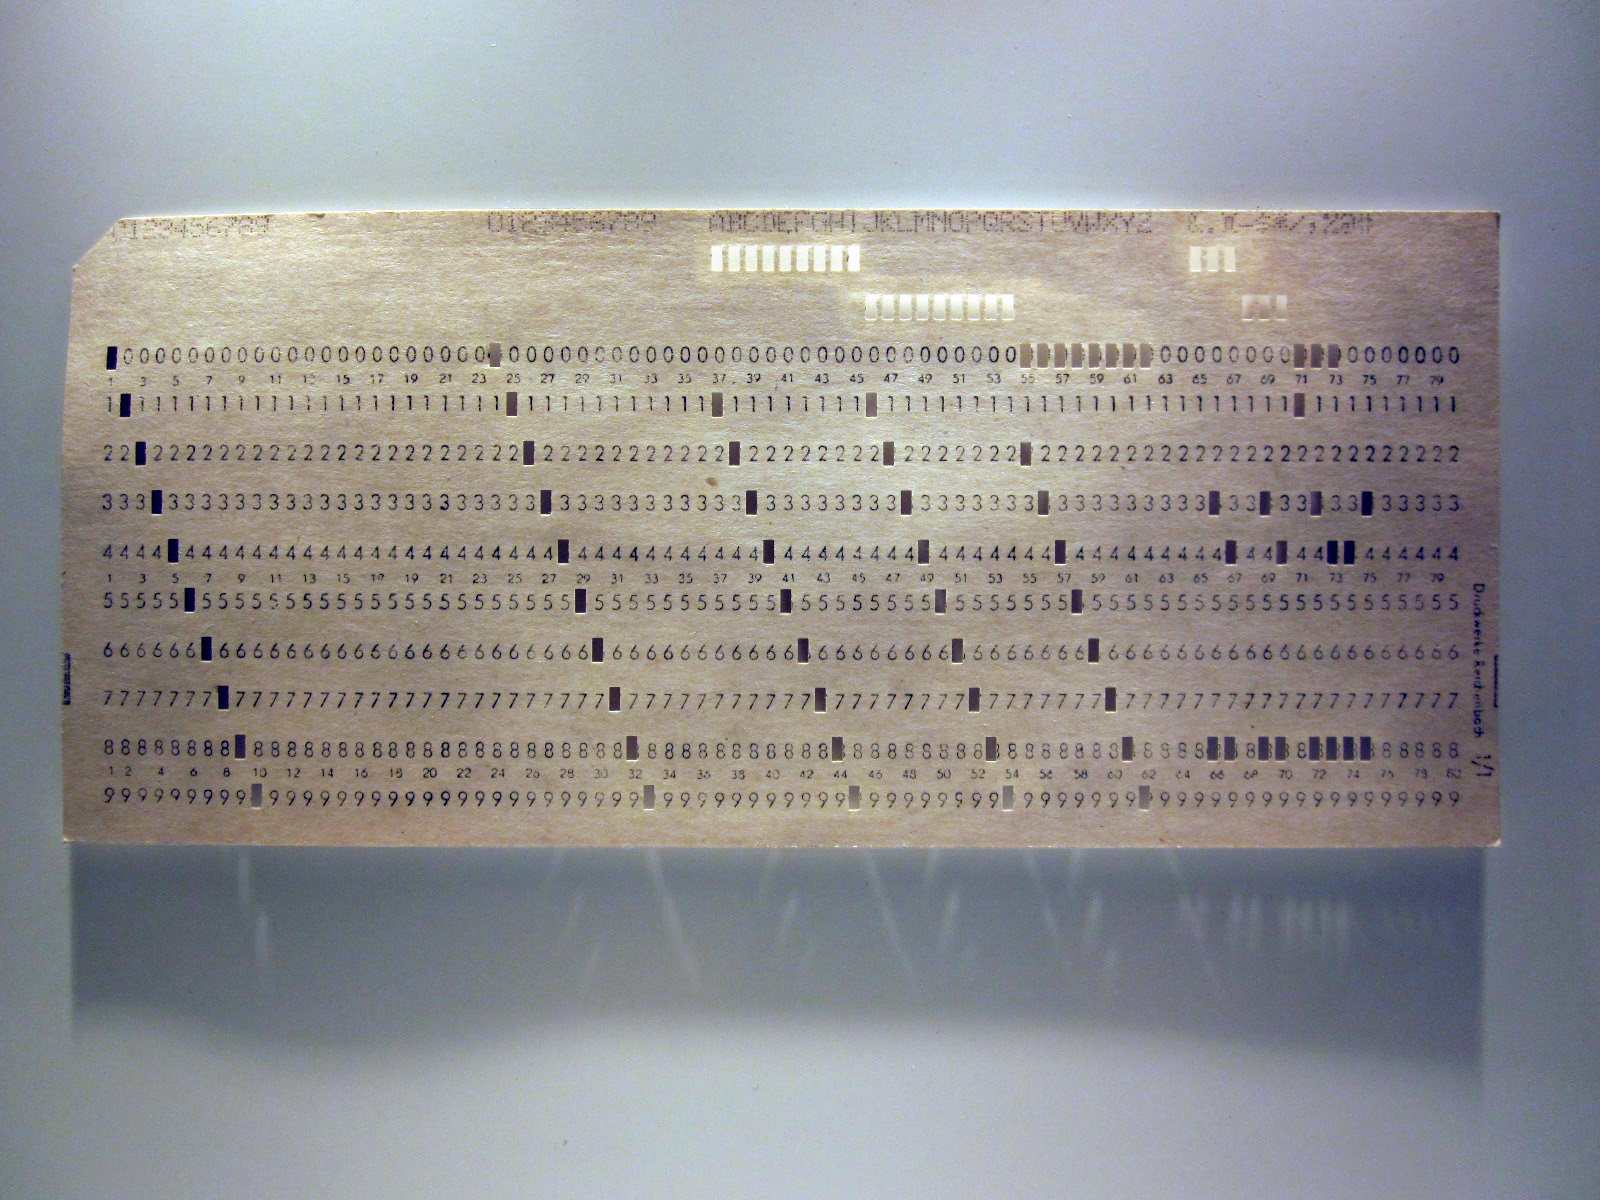
\includegraphics[width=0.6\textwidth]{fig/punchcard.jpg}
  \end{center}
  \smallurl{https://en.wikipedia.org/wiki/Punched_card}
\end{frame}
\begin{frame}
  \frametitle{From punch cards to transistors}
  
  \begin{minipage}{0.45\textwidth}
    \vspace{-1cm}
    Fortunately, we don't have to use punch cards anymore. Modern computers use billions of tiny \textbf{transistors} to store bits and execute instructions.
    \end{minipage}
    \begin{minipage}{0.5\textwidth}
    \vspace{-1cm}
    \begin{center}
      \vspace{0.5cm}
      AMD Athlon 64 3200+\\
      \smallskip
    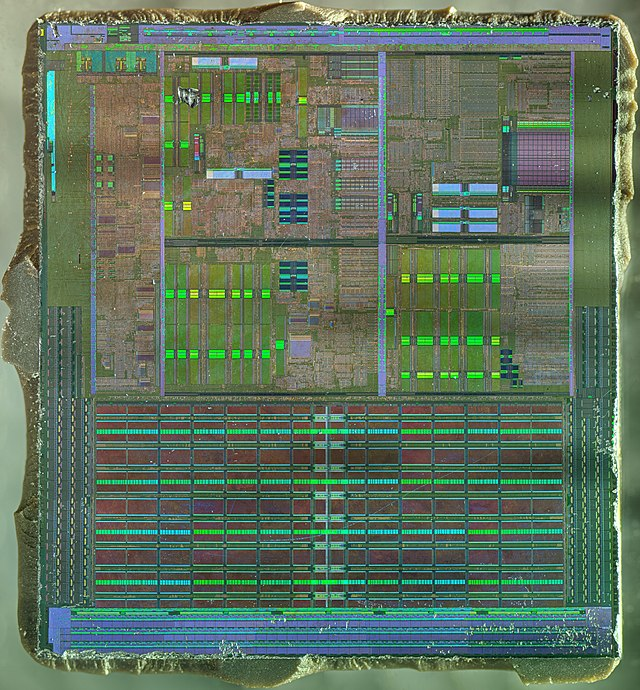
\includegraphics[width=0.85\textwidth]{fig/Athlon.jpg}
    \end{center}
    \smallurl{https://commons.wikimedia.org/wiki/File:Moores_law_\%281970-2011\%29.PNG}
    \end{minipage}
\end{frame}

\begin{frame}
  \frametitle{Moore's Law}

  \begin{minipage}{0.3\textwidth}
    \vspace{-1cm}
    \textbf{Moore's Law:}
    The number of transistors on a microchip doubles approximately every two years.
    \end{minipage}
    \begin{minipage}{0.68\textwidth}
    \vspace{-1cm}
    \begin{center}
    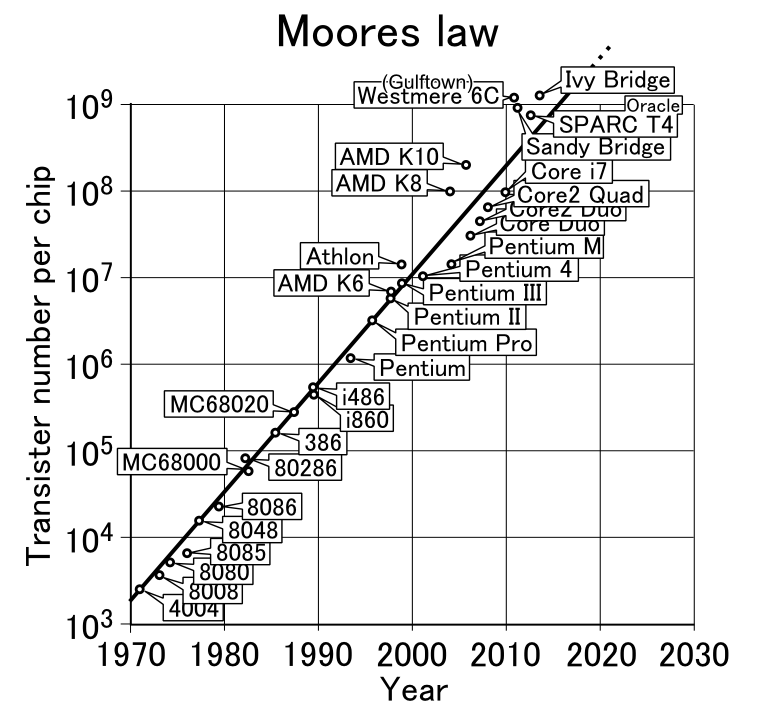
\includegraphics[width=\textwidth]{fig/Moores_law.png}
    \end{center}
    \vspace{-1cm}
    \smallurl{https://commons.wikimedia.org/wiki/File:Moores_law_\%281970-2011\%29.PNG}
    \end{minipage}
\end{frame}
\begin{frame}
  \frametitle{Computer Hardware}
  A computer consists of the following main components:
  \begin{itemize}
    \item \textbf{Central Processing Unit (CPU)}: The brain of the computer. It executes instructions.
    \item \textbf{Motherboard}: Main circuit board of the computer.
    \item \textbf{Memory}: RAM, ROM, hard disk, etc.
    \item \textbf{Input devices}: Keyboard, mouse, microphone, camera, etc.
    \item \textbf{Output devices}: Monitor, printer, speakers, etc.
    \item \textbf{Power supply}: Provides power to the computer.
    \item \textbf{Network interface}: For connecting to other networks.
  \end{itemize}
\end{frame}
\begin{frame}
  \frametitle{Central Processing Unit (CPU)}
  The CPU is the brain of the computer. It executes instructions which are stored in the memory.\\
  \vspace{5mm}
  \textbf{Instruction}: A command that the CPU can execute. \textsc{ADD}, \textsc{MOV}, \textsc{JMP}, etc. are examples of instructions.\\
  \textbf{Instruction set}: A set of instructions that the CPU can execute. Examples: \texttt{x86}, \texttt{ARM}\\
  \textbf{Registers}: Small amount of memory inside the CPU. The CPU can access the registers very quickly.\\
\end{frame}
\begin{frame}
  \frametitle{Motherboard}
  Facilitates communication between the CPU, memory, input devices, output devices, etc. and provides power to the components. \\
  \vspace{5mm}
  \textbf{BIOS}: Program which executes when the computer is turned on. It initializes the hardware and loads the operating system.\\
\end{frame}
\begin{frame}
  \frametitle{Memory}
  Computer memory is used to store data and instructions executed by the CPU.\\
  \vspace{5mm}
  Various types of memory are used in a computer: 
  \begin{itemize}
    \item \textbf{RAM}: Random Access Memory. (volatile)\\Stores data \& instructions that are currently being used by the CPU.
    \item \textbf{ROM}: Read Only Memory. (non-volatile)\\Stores the BIOS and other programs that are executed when the computer is turned on.
    \item \textbf{Disk}: HDD/SSD/Tape etc. (non-volatile)\\Used to store large amounts of data. 
  \end{itemize}
\end{frame}
\begin{frame}
  \frametitle{Input \& Output devices}
  Input and output devices are used to communicate with the computer.\\
  \vspace{5mm}
  Historically: keyboard, later mouse and touch screen. \\
  \vspace{5mm}
  Monitors CRTs: limited to 80 characters per line.\\
  \vspace{5mm}
  Nowadays: LCDs, OLEDs, etc.\\
\end{frame}
\begin{frame}
  \frametitle{Power supply \& Network interface}
  The power supply provides power to various components of the computer.\\
  \vspace{5mm}
  It converts the AC power from the outlet to DC power with various voltages (+3.3 V, +5 V and +12 V) required by the computer.\\
  \vspace{5mm}
  The network interface is used to connect the computer to other networks via various networking technologies (Ethernet, WiFi, etc.).\\
\end{frame}
\begin{frame}
  \frametitle{How to get a computer to do something?}
  Historically, computers were programmed using punch cards.\\
  \begin{center}
    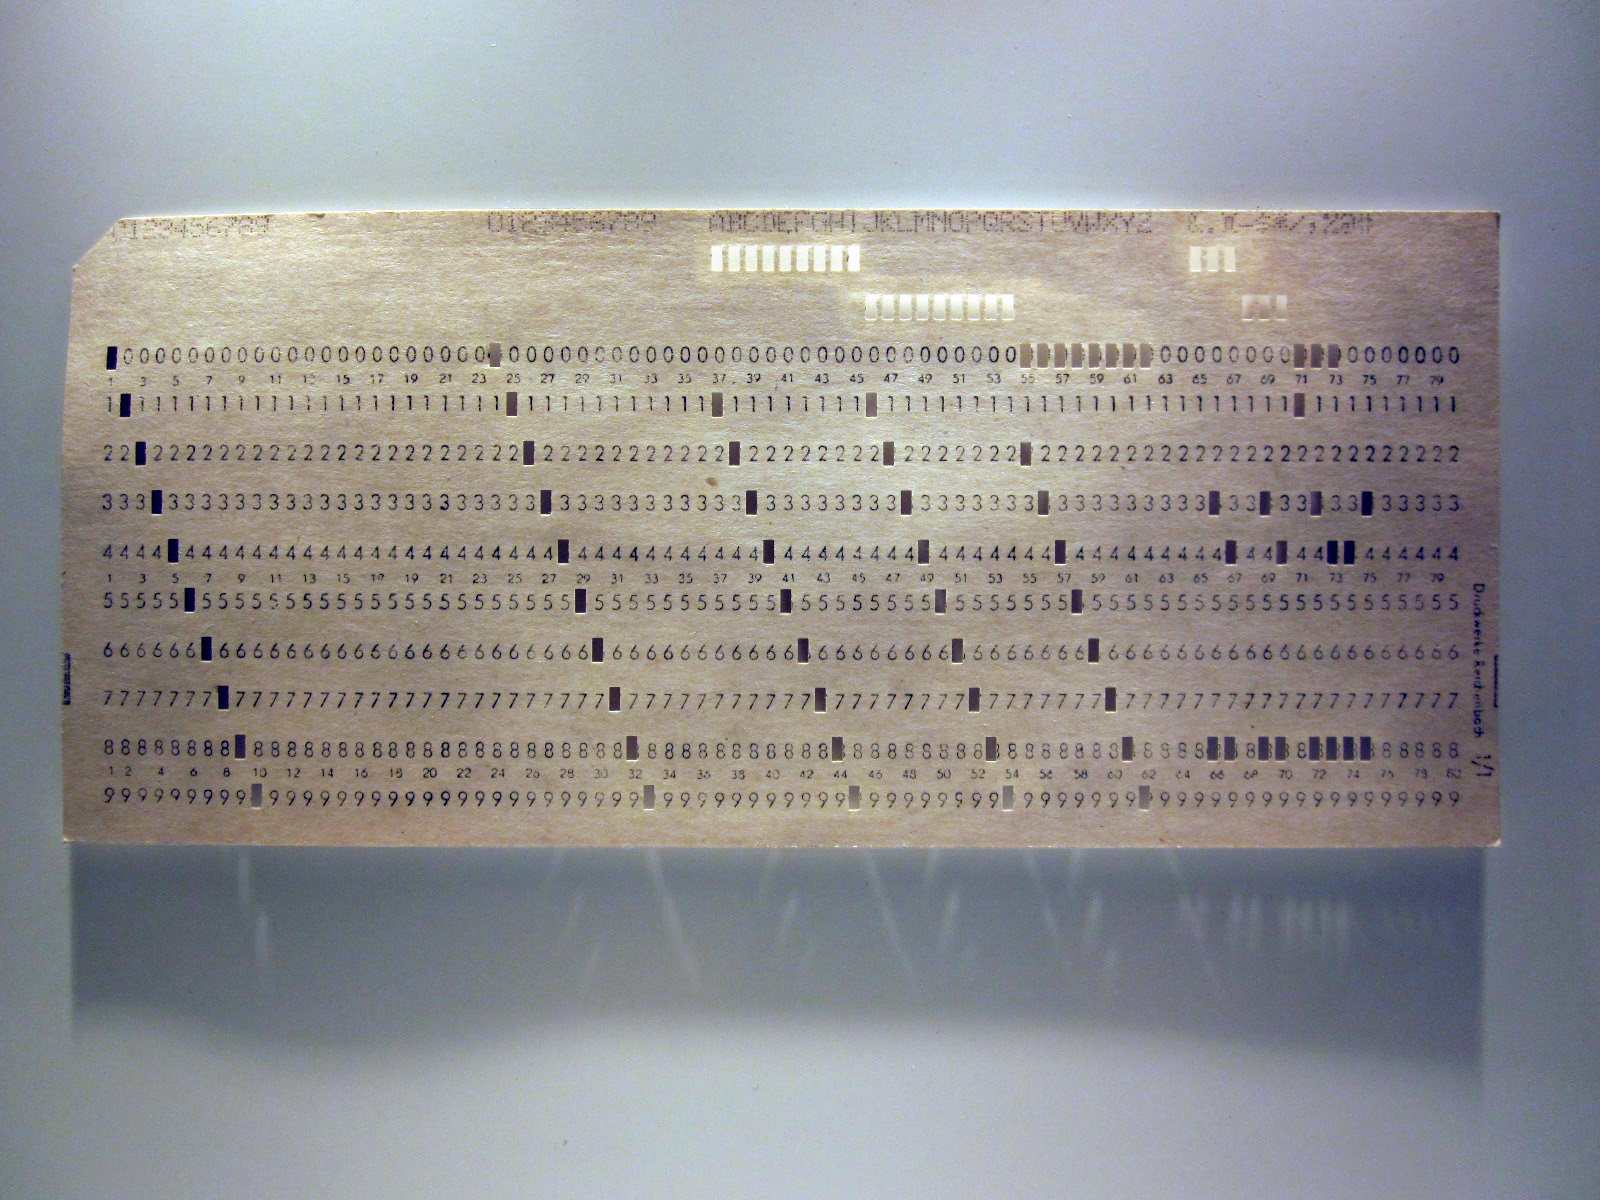
\includegraphics[width=0.5\textwidth]{fig/punchcard.jpg}
  \end{center}
  \smallurl{https://en.wikipedia.org/wiki/Punched_card}
\end{frame}
\begin{frame}
  \frametitle{How to get a computer to do something?}
  Nowadays, computers can be programmed using a variety of \textbf{programming language}.\\
  \vspace{5mm}
  \textbf{Software}: set of instructions and data that is executed by the hardware of the computer.\\
  \vspace{5mm}
  \textbf{Programming language}: A language that is used to write software.\\
\end{frame}

\begin{frame}
  \frametitle{Different levels of complexity}
  \begin{itemize}
    \item \textbf{Machine language}: The language of the computer. Lowest level language \& only language that the computer can understand. It is written in \textbf{binary}.
    \item \textbf{Assembly language}: It is written in a symbolic form that is easier to read and write than machine language. Yet still very close to machine language. 
    \item \textbf{High-level languages}: A language that is closer to human languages than machine language. It is written in a symbolic form that is easier to read and write than machine language. It is portable and can be run on different machines.
  \end{itemize}
\end{frame}
\begin{frame}
  \frametitle{High-level languages}
  Because Machine as well as Assembly code is cumbersome to write, \textbf{High-level languages} were first developed in the 1950s.\\
  \begin{itemize}
    \item \textbf{Fortran}: It was the first high-level language to be widely used. (1957)
    \item \textbf{C/C++}: It is the most widely used programming language. (1972 / 1985)
    \item \textbf{Java}: It is a general-purpose, concurrent, class-based, object-oriented language. (1995)
    \item \textbf{Python}: It is a general-purpose, high-level, interpreted, dynamic programming language. (1991)
  \end{itemize}

\end{frame}
\begin{frame}
  \frametitle{High-level languages timeline}
  \begin{center}
    \includegraphics[width=\textwidth]{fig/programming\_languages\_timeline.png}
  \end{center}
\smallurl{https://i0.wp.com/javaconceptoftheday.com/wp-content/uploads/2019/07/TimelineOfProgrammingLanguages.png?ssl=1}
\end{frame}
\begin{frame}
  \frametitle{Who is translating?}
  High level languages are translated into machine code by a \textbf{compiler}.\\
  \vspace{0.5cm}
  The compiler takes the text file containing the code and translates it into 0s and 1s that the computer can understand.\\
  \vspace{0.5cm}
  The compiler then creates an executable file (\textsc{.exe}) that can be run on the computer.\\
\end{frame}
\begin{frame}
  \frametitle{From compilers to interpreters}
  \textbf{Compilers} have some disadvantages. They can be slow to run, and they require the user to compile the code before it can be executed.\\
  This led to the development of \textbf{interpreters}, which execute code \textbf{directly} without the need for compilation. \\
  Interpreters are often used for scripting languages (like \texttt{python}) and for prototyping new code quickly.
\end{frame}
\begin{frame}
  \frametitle{Operating system}
  An operating system (Linux, Windows, Mac OS, etc.) is a software which manages the computer hardware and software resources and provides common services for computer programs.\\
  \vspace{5mm}
  Manages and hands out RAM-memory to programs.\\ 
  \vspace{5mm}
  Manages and hands out CPU-time to programs.\\
  \vspace{5mm}
  Provides abstraction of the hardware.\\
\end{frame}
\begin{frame}
  \vspace*{\fill}
  \begin{center}
    \begin{quote}
        ``Operating systems are the masterful illusionists, the fair referees, and the unifying glue that seamlessly blend the complexities of hardware and the intricacies of software, creating a harmonious dance between them'' - Daniel Gruss (modified)
    \end{quote}
\end{center}
\vspace*{\fill}
\end{frame}
\section{How do Computers communicate}
\begin{frame}
  \frametitle{How do Computers communicate?}
  Computers can communicate with other remote computer by using:\\
  \begin{itemize}
    \item \textbf{\hrefu{https://en.wikipedia.org/wiki/Ethernet}{Ethernet}}: Used to connect computers in a local network.
    \item \textbf{\hrefu{https://en.wikipedia.org/wiki/Wi-Fi}{WiFi}}: Wireless Fidelity. Used to connect computers in a local network.
    \item \textbf{\hrefu{https://en.wikipedia.org/wiki/Transmission_Control_Protocol}{TCP}/\hrefu{https://en.wikipedia.org/wiki/User_Datagram_Protocol}{UDP}}: Transmission Control Protocol / User Datagram Protocol. Used to transfer data over the internet.
    \item \textbf{\hrefu{https://en.wikipedia.org/wiki/Hypertext_Transfer_Protocol}{HTTP}}: HyperText Transfer Protocol. Used to transfer web pages.
  \end{itemize}
\end{frame}
\begin{frame}
  \frametitle{How do Computers communicate?}
  \dots they communicate locally using: \\
  \begin{itemize}
    \item \textbf{\hrefu{https://en.wikipedia.org/wiki/USB}{USB}}: Universal Serial Bus. Used to connect peripherals to a computer.
    \item \textbf{\hrefu{https://en.wikipedia.org/wiki/RS-232}{RS-232}}: Recommended Standard 232 (serial communication). Used to connect peripherals to a computer.
    \item \textbf{\hrefu{https://en.wikipedia.org/wiki/MIDI}{MIDI}}: Musical Instrument Digital Interface. Used to connect musical instruments to a computer.
  \end{itemize}
\end{frame}
\begin{frame}
  
  \begin{center}
    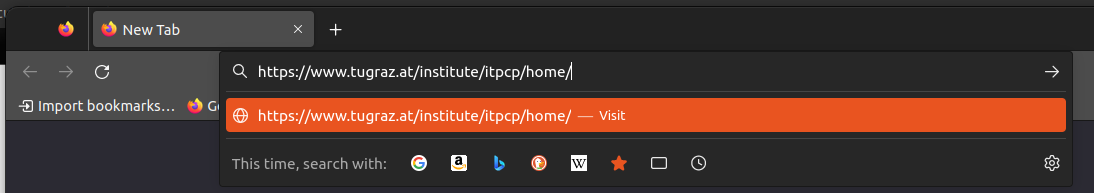
\includegraphics[width=\textwidth]{fig/search.png}
  \end{center}
  \begin{center}
    $\downarrow$ How does this work? $\downarrow$
  \end{center}
  \begin{center}
    \includegraphics[width=\textwidth]{fig/search\_result.png}
  \end{center}
\end{frame}
\begin{frame}
  \begin{center}
    \includegraphics[width=0.6\textwidth]{fig/osi\_model.png}
  \end{center}
  \vspace{-6mm}
  \smallurl{https://en.wikipedia.org/wiki/OSI\_model}
\end{frame}
\begin{frame}
  \frametitle{Let's look at a simplified example:}
  We want to access \texttt{\hrefu{www.tugraz.at/institute/itpcp/}{www.tugraz.at/institute/itpcp/}}\\
  \vspace{5mm}
  Our browser will send a \textbf{request} to the server at \texttt{\hrefu{www.tugraz.at}{www.tugraz.at}} using the \textbf{\hrefu{https://en.wikipedia.org/wiki/Hypertext_Transfer_Protocol}{HTTP}} protocol.\\
  \vspace{5mm}
  But how does he know where to send the request?\\
  \vspace{5mm}
  Computers have addresses, just like houses. They are called \textbf{\hrefu{https://en.wikipedia.org/wiki/IP\_address}{IP addresses}}.\footnote[frame]{\tiny actually it's more involved especially with IPv4 addresses $\rightarrow$ \hrefu{https://en.wikipedia.org/wiki/IPv4_address_exhaustion}{IPv4-exhaustion}}\\ % :( simplified i guess
\end{frame}
\begin{frame}
  \frametitle{IPv4 addresses}
  \begin{center}
    \includegraphics[width=\textwidth]{fig/ipv4\_config.png}
  \end{center}
  \vspace{-6mm}
\smallurl{https://www.flickr.com/photos/johnlsloan/5477351098}
\end{frame}
\begin{frame}
  \frametitle{How to get an IP address for a website?}
  Just ask another server for it $\rightarrow$ \textbf{\hrefu{https://en.wikipedia.org/wiki/Domain_Name_System}{DNS request}}
  \vspace{5mm}
  The request will be send from your computers network card to your router.\\ The router will forward the request to your ISP (Internet Service Provider; A1, Magenta, etc.).\\
  Maybe your ISP knows the IP address of the website, but if not, he will ask another server.\\
  \vspace{5mm}
  In case your ISP doesn't know the address, the request will be forwarded to the \textbf{\hrefu{https://en.wikipedia.org/wiki/Root\_name\_server}{root name server}}.\\
\end{frame}
\begin{frame}
  \frametitle{Root name server -- CERN Meyrin}
  \begin{center}
    \includegraphics[width=\textwidth]{fig/root\_server.jpg}
  \end{center}
  \smalltext{Foto: Elias Wachmann}
\end{frame}
\begin{frame}
  \frametitle{Now finally \dots}
  The root name server will send the IP address back to your ISP, which will send it back to your router, which will send it back to your computer.\\
  \vspace{5mm}
  Your computer now knows the address of the \texttt{\hrefu{www.tugraz.at}{www.tugraz.at}} server and can send the actual request to load \texttt{\hrefu{www.tugraz.at/institute/itpcp/}{www.tugraz.at/institute/itpcp/}}\\
  \vspace{5mm}
  The server will send the requested website back to your computer, which will display it in your browser.\\
\end{frame}

\section{Software Survival Kit}
\begin{frame}
  \frametitle{Software Survival Kit}
  This guide is a collection of useful information to use a computer to its full potential based on the lecture \hrefu{https://missing.csail.mit.edu/}{The Missing Semester of Your CS Education} by MIT.\\
  \vspace{5mm}
  \textbf{Video lectures} for the various topics can be found \hrefu{https://www.youtube.com/watch?v=Z56Jmr9Z34Q&list=PLyzOVJj3bHQuloKGG59rS43e29ro7I57J}{here}.\\
\end{frame}
\begin{frame}
  \frametitle{Shell \hrefu{https://www.youtube.com/watch?v=Z56Jmr9Z34Q&list=PLyzOVJj3bHQuloKGG59rS43e29ro7I57J}{[video]}}
  The shell is a program that takes commands from the keyboard and executes corresponding programs which are preinstalled with the OS.\\
  \begin{center}
    \includegraphics[width=0.75\textwidth]{fig/shell\_empty.png}
  \end{center}
Empty shell with \texttt{user}@\texttt{hostname}:\texttt{directory}\$
\end{frame}
\begin{frame}
  \frametitle{Shell -- echo}
  A simple example is \texttt{echo}:prints its arguments to the standard output.\\
  \begin{center}
    \includegraphics[width=0.75\textwidth]{fig/hello\_shell.png}
  \end{center}
  How can the shell know where to find the program \texttt{echo}?\\
  \vspace{5mm}
  \textbf{PATH}: A list of directories where the shell looks for programs.\\
\end{frame}
\begin{frame}
  \frametitle{Shell -- \$PATH}
  Let's look at the \texttt{PATH} variable.\\
  \begin{center}
    \includegraphics[width=\textwidth]{fig/shell\_path.png}
  \end{center}
  Echo prints out the value of the \texttt{\$PATH} variable.\\
  \texttt{\$PATH} includes the \texttt{/usr/bin} where echo is located.\\
  % \vspace{5mm}
  \begin{center}
    \includegraphics[width=\textwidth]{fig/shell\_which.png}
  \end{center}
\end{frame}
\begin{frame}
  \frametitle{Shell -- Directories}
  \textbf{Directories}: A directory is a file that contains a list of other files and directories.\\
  \textbf{Absolute path}: The full path to a file or directory.\\
  \textbf{Relative path}: The path to a file or directory relative to the current directory.\\
  \vspace{5mm}
  Change the current directory with \texttt{cd}.\\
  \begin{center}
    \includegraphics[width=\textwidth]{fig/shell\_cd.png}
    \texttt{cd ./directory} relative -- \texttt{cd /mnt/directory} absolute -- \texttt{cd ..} go back  
  \end{center}
\end{frame}
\begin{frame}
  \frametitle{Shell -- ls}
  \textbf{ls}: List directory contents.\\
  \begin{center}
    \includegraphics[width=\textwidth]{fig/shell\_ls.png}
   \end{center}
\end{frame}
\begin{frame}
  \frametitle{Need more information?}
  No problem! Just type: \texttt{man} followed by the program name: 
  \begin{center}
    \includegraphics[width=\textwidth]{fig/shell\_man.png}
   \end{center}
\end{frame}
\begin{frame}
  \frametitle{Shell -- try it out yourself}
  Lecture notes can be found \hrefu{https://missing.csail.mit.edu/2020/course-shell/}{here}.\\
  \vspace{5mm}
  Feel free to try out some exercises on the page to get familiar with the shell.\\
\end{frame}
\begin{frame}
  \frametitle{Git}

  

\end{frame}
\begin{frame}
  \frametitle{Git [\hrefu{https://www.youtube.com/watch?v=2sjqTHE0zok&t=1s}{video}]}
  Git is a version control system.\\
  \vspace{5mm}
  \textbf{Version control system}: A system that records changes to a file or set of files over time so that you can recall specific versions later.\\
  \vspace{5mm}
  \textbf{But why should I use it?}\\
  No more \texttt{report\_v1\_final\_final\_final\_final.pdf}!\\
  \vspace{5mm}
  You can download git \hrefu{https://git-scm.com/downloads}{here}.
\end{frame}

\begin{frame}
  \frametitle{Git -- initializes a new repository (init)}
  \textbf{Repository}: A directory where git has been initialized to start version controlling your files.\\
  \vspace{5mm}
  To initializes a new repository use \texttt{git init}.\\
  \begin{center}
    \includegraphics[width=\textwidth]{fig/git\_init.png}
   \end{center}
  This creates a hidden folder \texttt{.git} which contains all the information about the repository.\\
\end{frame}
\begin{frame}
  \frametitle{Git -- add files (add)}
  To add files to the repository use \texttt{git add}.\\
  This stages the files for the next commit. 
  \begin{center}
    \includegraphics[width=\textwidth]{fig/git\_add.png}
   \end{center}
  Here ''Hello World'' is redirected into a file called \texttt{testfile.txt} using the \texttt{>} operator.\\
  All files in the current folder and in subfolder bellow can be added using \texttt{git add .} (with a fullstop).\\
\end{frame}
\begin{frame}
  \frametitle{Git -- see current status (status)}
  To see the current status of the repository use \texttt{git status}.\\
  \begin{center}
    \includegraphics[width=\textwidth]{fig/git\_status.png}
   \end{center}
  \texttt{testfile.txt} is staged for commit.\\
\end{frame}
\begin{frame}
  \frametitle{Git -- commit changes (commit)}
  To commit the changes use \texttt{git commit}.\\
  \begin{center}
    \includegraphics[width=\textwidth]{fig/git\_commit\_fail.png}
  \end{center}
  That didn't work $\rightarrow$ setup your git user name \& email.\\
\end{frame}
\begin{frame}
  \frametitle{Git -- setup user name \& email (config)}
  To setup your user name \& email use \texttt{git config}.\\
  The \texttt{--global} flag sets the configuration (globally) for the current user.\\
  \begin{center}
    \includegraphics[width=\textwidth]{fig/git\_commit.png}
  \end{center}
  After setting up the user name \& email you can commit the changes.\\
  Commit messages should be short and meaningful and can be added using the \texttt{-m} flag.\\
\end{frame}
\begin{frame}
  \frametitle{Git -- see commit history (log)}
  To see the commit history use \texttt{git log}.\\
  \begin{center}
    \includegraphics[width=\textwidth]{fig/git\_log.png}
  \end{center}
  Each commit has a unique identifier called a \textbf{SHA}.\\
  This allows you to go back to a specific commit.\\
\end{frame}
\begin{frame}
  \frametitle{Git -- Remote repositories}
  \textbf{Remote repository}: A repository that is hosted on the Internet or another network.\\
  \vspace{5mm}
  It is a good idea to have a remote repository to backup your work or collaborate with others.\\
  \vspace{5mm}
  \textbf{GitLab}: A website that hosts git repositories (relevant for the exercises later).\\
\end{frame}
\begin{frame}
  \frametitle{Git -- Remote (remote)}
  To add a remote repository use \texttt{git remote} followed by an alias and \texttt{url}.\\
  \begin{center}
    \includegraphics[width=\textwidth]{fig/git\_remote\_add.png}
   \end{center}
  Here \texttt{origin} is used as a remote alias and \texttt{../remote/} as the url. \\
\end{frame}
\begin{frame}
  \frametitle{Git -- Remote (clone)}
  To clone a remote repository use \texttt{git clone} followed by the \texttt{url}.\\
  The url can be found on the gitlab page of the repository.\\
  \begin{center}
    \includegraphics[width=\textwidth]{fig/git\_remote\_clone.png}
  \end{center}
\end{frame}
\begin{frame}
  \frametitle{Git -- Remote (push \& pull)}
  When cloning a repository the remote alias \texttt{origin} is automatically added.\\
  All changes are loaded into the local repository.\\
  \vspace{5mm}
  After working on the project locally you can push the changes to the remote repository using \texttt{git push}.\\
  \vspace{5mm}
  \textbf{Note}: You can also pull changes from a remote repository using \texttt{git pull}.\\
\end{frame}
\begin{frame}
  \frametitle{Git -- SSH keys?}
  \textbf{SSH}: Secure Shell (SSH) is a cryptographic network protocol for operating network services securely over an unsecured network.\\
  \vspace{5mm}
  \textbf{SSH keys}: An SSH key is an access credential in the SSH protocol.\\
  \vspace{5mm}
  \textbf{You need to setup SSH keys to push changes to a remote repository.}\\
  \vspace{5mm}
  Use \hrefu{https://docs.gitlab.com/ee/user/ssh.html\#generate-an-ssh-key-pair}{this Guide} to setup \hrefu{https://docs.gitlab.com/ee/user/ssh.html\#add-an-ssh-key-to-your-gitlab-account}{link} your SSH keys to GitLab.\\
\end{frame}

\begin{frame}
  \frametitle{Git -- Branches}
  \textbf{Branch}: A branch is a parallel version of a repository.\\
  \vspace{5mm}
  \textbf{Main branch}: The default branch when you create a repository.\\
  \vspace{5mm}
  You can create a new branch using \texttt{git branch} followed by the branch name.\\
  \vspace{5mm}
  You can switch to a branch using \texttt{git switch} followed by the branch name.\\
\end{frame}
\begin{frame}
  \frametitle{Git -- Branches (merge)}
  To \textbf{merge} a branch into the main branch use \texttt{git merge} followed by the branch name.\\
  This will merge the changes from the branch into the main branch.\\
  \vspace{5mm}
  \textbf{Beware of conflicts!}\\
  \vspace{5mm}
  If you and another person change the same line of code, git will not know which change to keep $\rightarrow$ a merge conflict will occur which must be resolved manually.\\
\end{frame}
\begin{frame}
  \frametitle{Need more information?}
  No problem! Just type: \texttt{git help} followed by a git command: 
  \begin{center}
    \includegraphics[width=\textwidth]{fig/git\_help.png}
   \end{center}
\end{frame}
\begin{frame}
  \frametitle{Git -- PRACTICE!!!}
  That was a lot of information.\\
  However, \textbf{git} can make your life a lot easier!\\
  \vspace{5mm}
  Invest some time and save a lot of time in the future: 
  \begin{itemize}
    \item \hrefu{https://www.codecademy.com/learn/learn-git}{Learn Git \& GitHub}
    \item \hrefu{https://learngitbranching.js.org/}{Learn Git Branching}
    \item \hrefu{https://ohmygit.org/}{Learn Git interactively}
    \item \hrefu{https://www.atlassian.com/git/tutorials/using-branches/git-merge}{Merging in Git}
  \end{itemize}

  

\end{frame}
%
\section{Additional Resources}
\begin{frame}
  \frametitle{Additional Resources}
  \begin{itemize}
    \item \hrefu{https://www.codewars.com/}{Codewars}
    \item \hrefu{https://leetcode.com/}{Leetcode}
    \item \hrefu{https://ohmygit.org/}{Oh my git!}
    \item \hrefu{https://www.learnpython.org/}{Interactive python tutorials}
    \item \hrefu{https://www.codecademy.com/learn/learn-python-3}{Learn Python 3}
    \item \hrefu{https://pll.harvard.edu/course/cs50-introduction-computer-science?delta=0}{CS50}
  \end{itemize}
   

\end{frame}

%-> 06-GIT
%-> optional Debugging 07-Debugging
%!Todo ASCII beschreiben
%!Todo ASCII Tabelle
% Illusionist
%%%%%%%%%%%%%%%%%%%%%%%%%%%%%%%%%%%%%%%%%%%%%%%%%%%%%%%%%%%%%%%%%%%%%%%%%%%%

\end{document}
%%%%%%%%%%%%%%%%%%%%%%%%%%%%%%%%%%%%%%%%%%%%%%%%%%%%%%%%%%%%%%%%%%%%%%%%%%%%

%% EOF

